{
\newcommand{\myscale}{0.6}
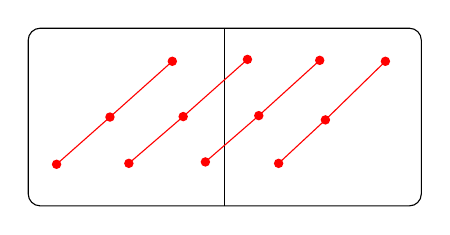
\begin{tikzpicture}[scale=\myscale, every node/.style={scale=\myscale}]
        \def\xscale{1.0} % Horizontal scale factor
        \def\yscale{1.0} % Vertical scale factor
        \def\spnt{0.1} % Size of smaller points
        \def\lpnt{0.125} % Size of larger points
        \def\roundscale{0.5} % The rounding factor
        \draw[rounded corners=2ex*\roundscale] (0,0) rectangle (8.32*\xscale,3.76*\yscale);
        \draw (4.16*\xscale, 3.76*\yscale) -- (4.16*\xscale, 0);
        \fill[red] (0.6*\xscale, 0.88*\yscale) circle (\spnt);
        \fill[red] (1.73*\xscale, 1.88*\yscale) circle (\spnt);
        \fill[red] (3.05*\xscale, 3.06*\yscale) circle (\spnt);
        \draw[red] (0.6*\xscale, 0.88*\yscale) -- (1.73*\xscale,1.88*\yscale) -- (3.05*\xscale,3.06*\yscale);
        \fill[red] (2.13*\xscale, 0.9*\yscale) circle (\spnt);
        \fill[red] (3.28*\xscale, 1.89*\yscale) circle (\spnt);
        \fill[red] (4.64*\xscale, 3.1*\yscale) circle (\spnt);
        \draw[red] (2.13*\xscale, 0.9*\yscale) -- (3.28*\xscale,1.89*\yscale) -- (4.64*\xscale,3.1*\yscale);
        \fill[red] (3.75*\xscale, 0.93*\yscale) circle (\spnt);
        \fill[red] (4.88*\xscale, 1.91*\yscale) circle (\spnt);
        \fill[red] (6.17*\xscale, 3.08*\yscale) circle (\spnt);
        \draw[red] (3.75*\xscale, 0.93*\yscale) -- (4.88*\xscale,1.91*\yscale) -- (6.17*\xscale,3.08*\yscale);
        \fill[red] (5.3*\xscale, 0.9*\yscale) circle (\spnt);
        \fill[red] (6.29*\xscale, 1.82*\yscale) circle (\spnt);
        \fill[red] (7.56*\xscale, 3.06*\yscale) circle (\spnt);
        \draw[red] (5.3*\xscale, 0.9*\yscale) -- (6.29*\xscale,1.82*\yscale) -- (7.56*\xscale,3.06*\yscale);
\end{tikzpicture}
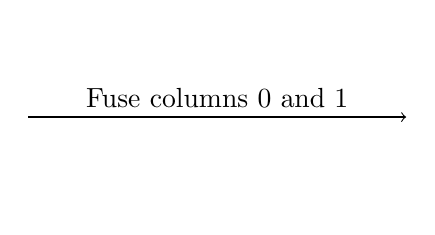
\begin{tikzpicture}[scale=\myscale, every node/.style={scale=1}]
    \draw[white] (0,0) rectangle (2,3.76);
    \draw[->] (-3,1.88) -- (5,1.88) node[above,pos=.5] {Fuse columns $0$ and $1$};
\end{tikzpicture}
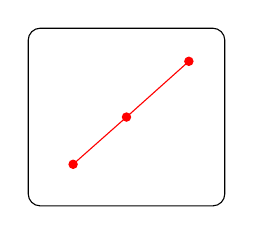
\begin{tikzpicture}[scale=\myscale, every node/.style={scale=\myscale}]
        \def\xscale{1.0} % Horizontal scale factor
        \def\yscale{1.0} % Vertical scale factor
        \def\spnt{0.1} % Size of smaller points
        \def\lpnt{0.125} % Size of larger points
        \def\roundscale{0.5} % The rounding factor
        \def\sh{0.35}
        \draw[rounded corners=2ex*\roundscale] (0,0) rectangle (4.16*\xscale,3.76*\yscale);
        \fill[red] ({(\sh+0.6)*\xscale}, 0.88*\yscale) circle (\spnt);
        \fill[red] ({(\sh+1.73)*\xscale}, 1.88*\yscale) circle (\spnt);
        \fill[red] ({(\sh+3.05)*\xscale}, 3.06*\yscale) circle (\spnt);
        \draw[red] ({(\sh+0.6)*\xscale}, 0.88*\yscale) -- ({(\sh+1.73)*\xscale},1.88*\yscale) -- ({(\sh+3.05)*\xscale},3.06*\yscale);
\end{tikzpicture}
}